\documentclass{article}
\usepackage{amsmath}
\usepackage{amsfonts}
\usepackage{amssymb}
\usepackage{amsthm}
\usepackage{geometry}
\usepackage{algorithm}
\usepackage{algpseudocode}
\usepackage{minted}
\usepackage{graphicx}
\usepackage{booktabs}
\usepackage{caption}
\usepackage{xcolor}
% \usepackage{subcaption}

\geometry{a4paper, left=2cm, right=2cm, top=2cm, bottom=2cm}

\title{Report for AI Capstone Homework 3: A Robot Navigation Framework}
\author{FU, YONG-WEI (112550107)}
\date{\today}

\begin{document}

\maketitle

\section{Implementation}

\subsection{Code explanation}
My pipeline is composed of several modules, and there are four of them I want to dig into:

\subsubsection{load\_and\_filter\_map()}

\begin{figure}[H]
    \centering
    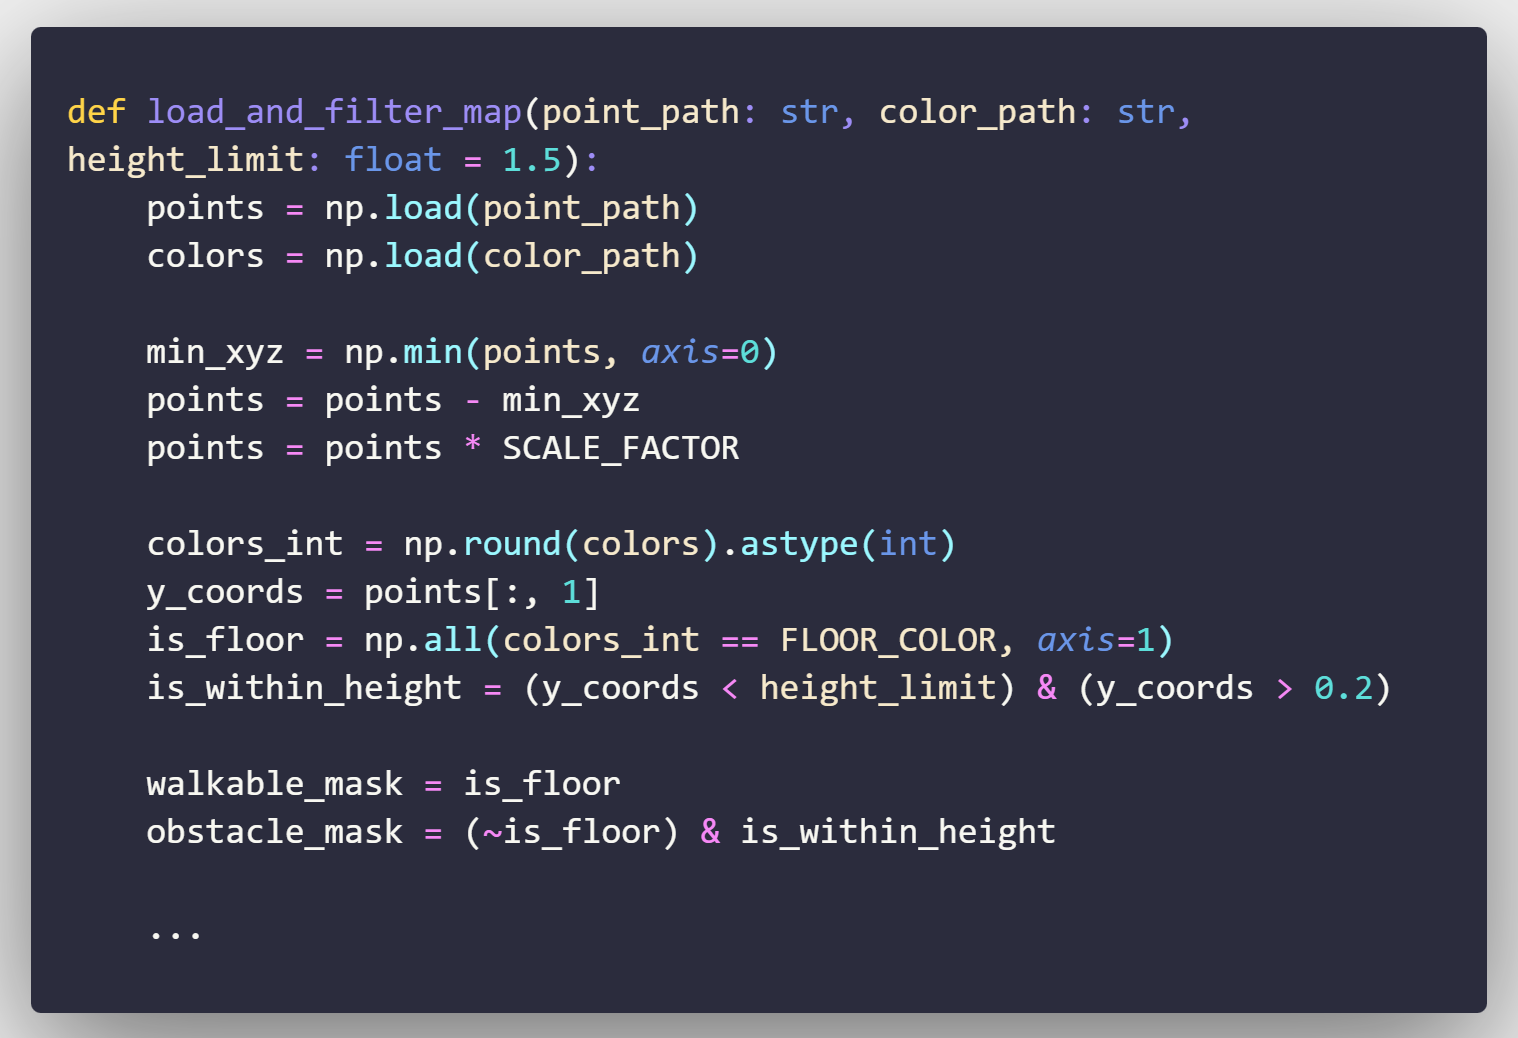
\includegraphics[width=0.9\textwidth]{polacode/load_and_filter_map.png} 
    \caption{Implementation of the 3D point cloud processing and filtering logic.}
    \label{fig:load_filter_code}
\end{figure}

The \texttt{load\_and\_filter\_map()} function converts raw 3D point cloud data into a 
2D navigation grid.

\begin{itemize}
    \item \textbf{Coordinate Transformation:} Raw points are shifted into the 
    positive quadrant and then scaled using a \texttt{SCALE\_FACTOR} to convert 
    them into real-world units first.
    \item \textbf{Mask Filtering:} I filter points into two masks 
    (\texttt{walkable\_mask} and \texttt{obstacle\_mask}) based on their semantic 
    colors and vertical $Y$-axis coordinates. Specifically, I extracted the 
    \texttt{walkable\_mask} based strictly on the semantic floor color, 
    and defined the \texttt{obstacle\_mask} by identifying points that are \textbf{not} 
    the floor and fall within a specific vertical range ($0.2m < y < 1.5m$). 
    This ensures the robot ignores the ground it stands on while capturing all 
    physical barriers that exist within its height clearance.
    \item \textbf{2D Projection:} The 3D $(x, y, z)$ points are projected onto 
    a 2D $(x, z)$ grid with a resolution of $0.05m$ per pixel.
    \item \textbf{Morphological Processing:} I use \texttt{cv2.morphologyEx} with 
    a kernel to fill gaps in the floor map (caused by sparse point cloud data). I also 
    use \texttt{cv2.dilate} on the occupancy map to add a safety margin around obstacles, 
    ensuring the RRT does not plan paths too close to walls.
\end{itemize}

\subsubsection{pick\_goal()}

\begin{figure}[H]
    \centering
    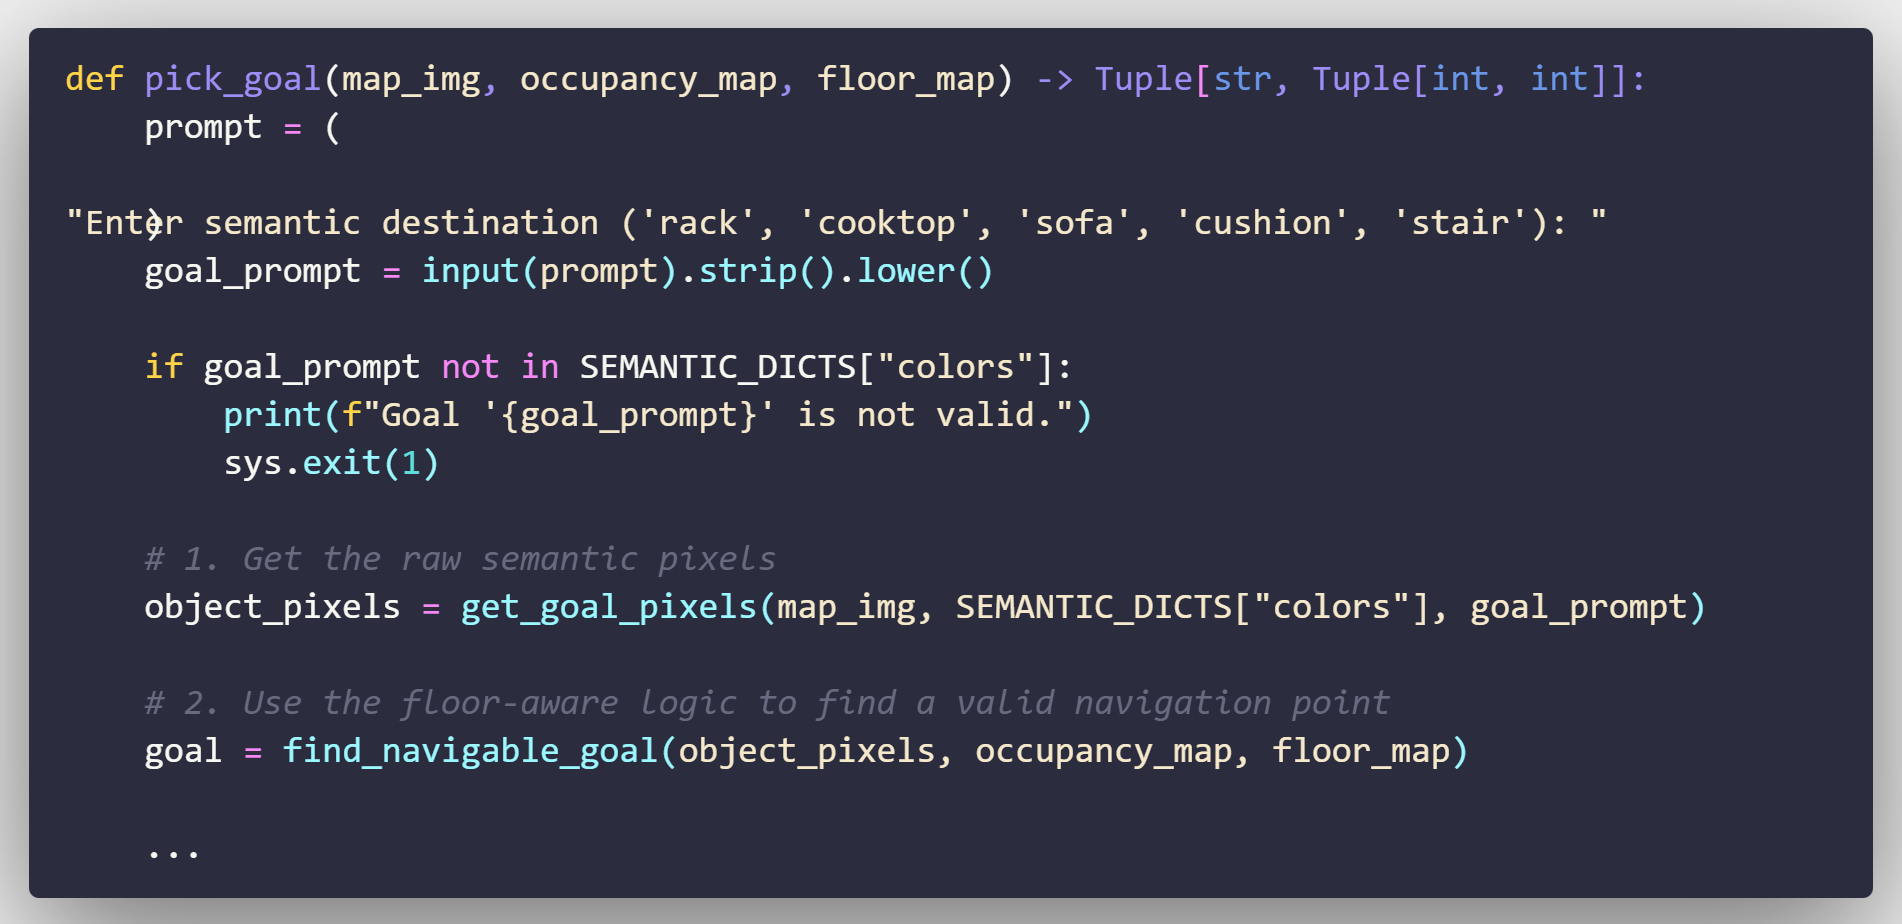
\includegraphics[width=0.9\textwidth]{polacode/pick_goal.png}
    \caption{Code snippet showing the goal selection and distance transform logic.}
    \label{fig:pick_goal_code}
\end{figure}

The \texttt{pick\_goal()} function and its helpers translate a user's semantic text command into a precise, 
reachable coordinate on the 2D grid.

\begin{itemize}
    \item \textbf{Semantic Color Matching:} The \texttt{get\_goal\_pixels()} function 
    iterates through the normalized RGB values defined in \texttt{SEMANTIC\_DICTS}. It 
    identifies all pixels in the \texttt{map\_img} that match the target furniture and returns it.
    \item \textbf{Distance Transform for Clearance:} To ensure the robot doesn't get 
    stuck in a ``dead zone'' (pixels too close to obstacles to be reachable by RRT and the robot), 
    I used \texttt{cv2.distanceTransform} to calculate the Euclidean distance 
    from every free pixel to the nearest obstacle. By requiring a \texttt{SAFE\_DISTANCE} of 
    at least 5 pixels, the algorithm filters out narrow gaps and ``edge pixels'' that would 
    otherwise cause navigation failures.
    \item \textbf{Centroid-based Navigation Point:} Instead of picking a random pixel 
    on the object's surface, the algorithm calculates the \textbf{centroid} $(\bar{x}, \bar{z})$ 
    of all identified pixels of that object. This provides a stable reference point in the ``center'' 
    of the furniture.
    \item \textbf{Nearest Safe Floor Selection:} The final goal is determined by finding 
    the pixel that is:
    \begin{enumerate}
        \item Labeled as floor in the \texttt{floor\_map}.
        \item Marked as free space in the \texttt{occupancy\_map}.
        \item Verified to have sufficient clearance via the distance transform.
    \end{enumerate}
    The algorithm uses \texttt{np.hypot} to calculate the distance from the object's centroid to 
    all ``safe'' floor candidates and selects the one with the minimum distance. This ensures the 
    robot stops directly in front of the target furniture when navigating.
\end{itemize}

\subsubsection{plan\_path()}

\begin{figure}[H]
    \centering
    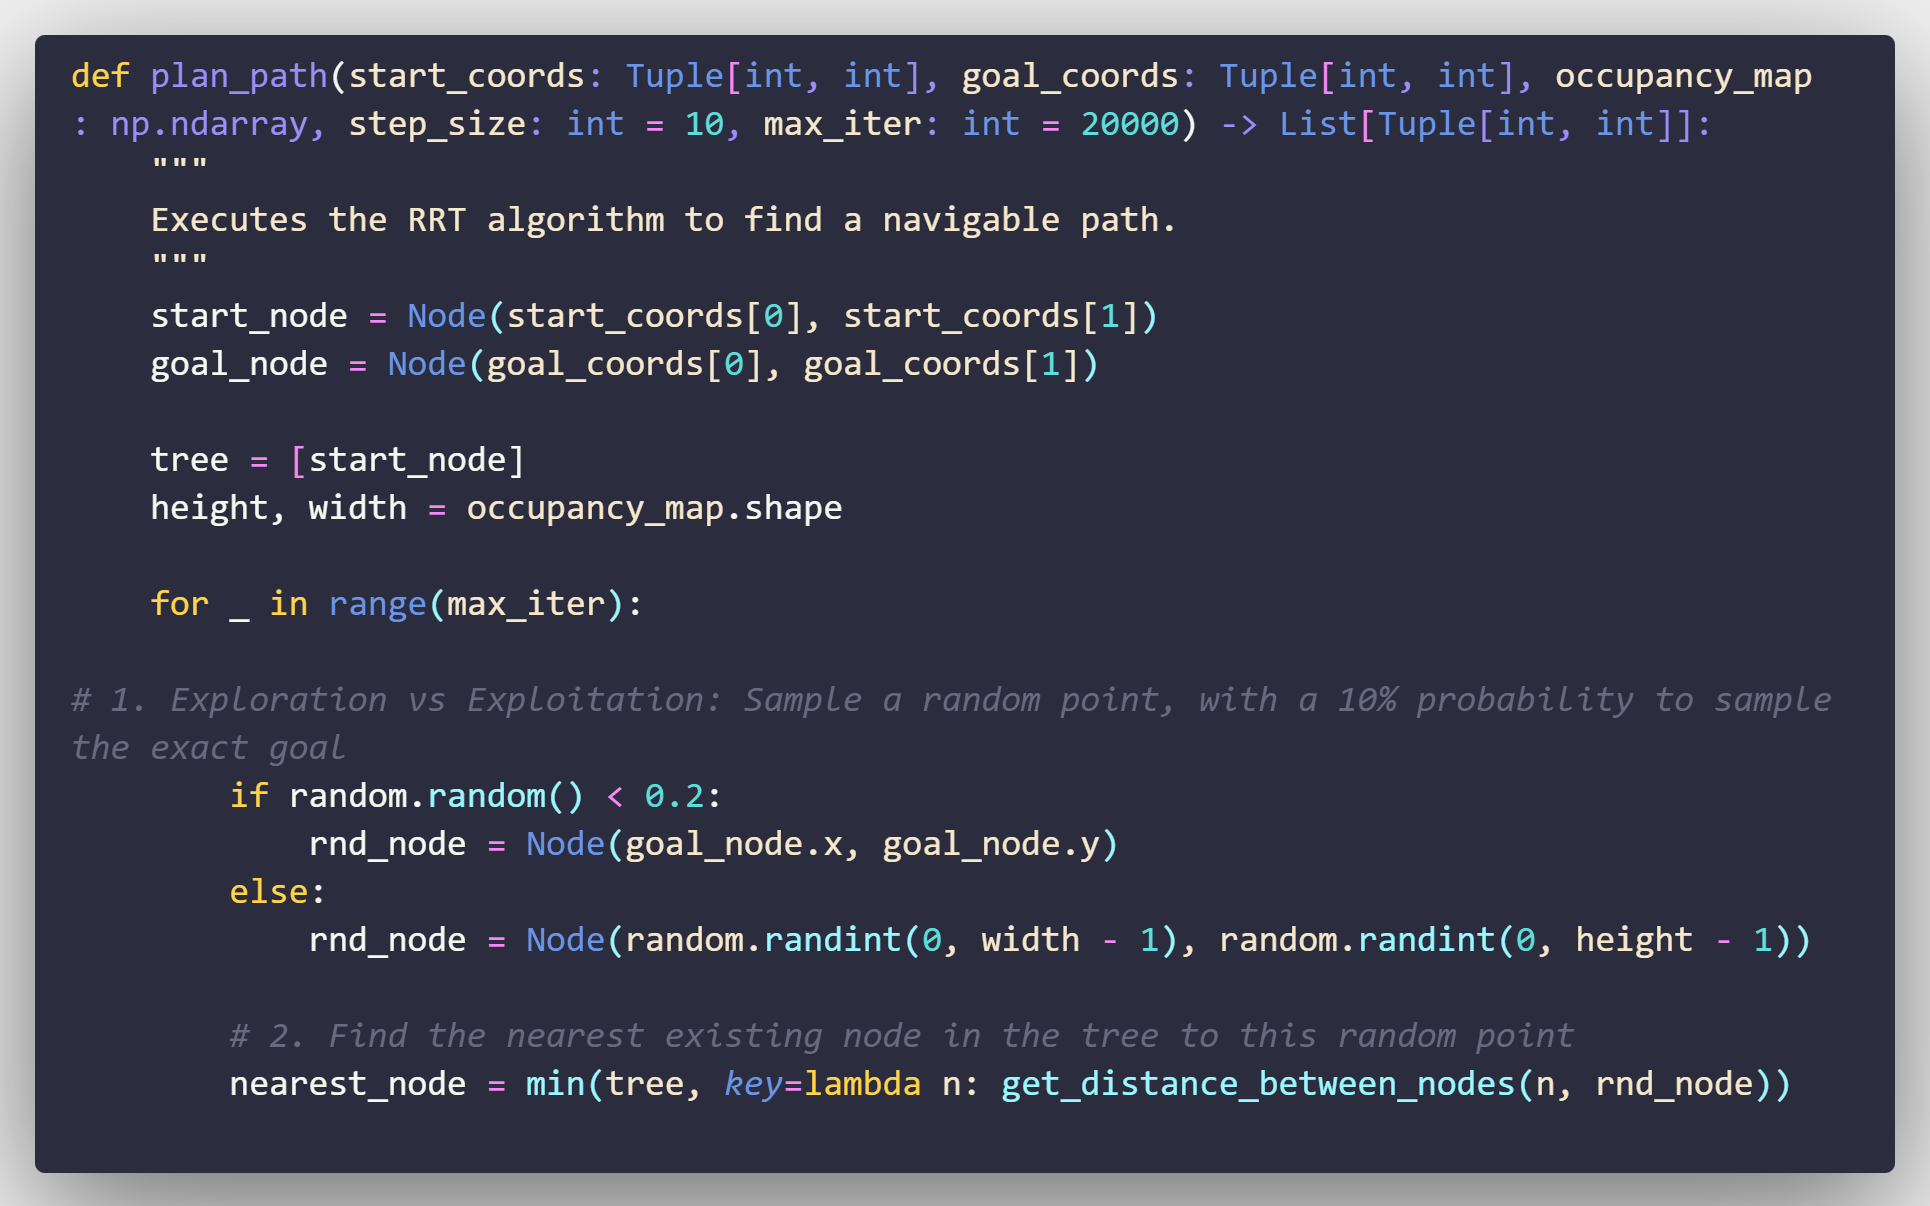
\includegraphics[width=0.9\textwidth]{polacode/plan_path.png}
    \caption{RRT path planning implementation featuring goal-biasing and collision checking.}
    \label{fig:plan_path}
\end{figure}

The \texttt{plan\_path()} function implements the core Rapidly-exploring Random 
Tree (RRT) algorithm to navigate the 2D occupancy grid. It iteratively grows a 
tree from the start position until it successfully connects to the target goal.

\begin{itemize}
    \item \textbf{Biased Sampling (Exploration vs. Exploitation):} To balance the search 
    between exploring the entire map and moving directly toward the target, the algorithm 
    uses a $20\%$ goal bias. In each iteration, there is a $20\%$ chance the goal itself is 
    sampled as the target point, while the remaining $80\%$ of the time a random coordinate 
    is chosen from the entire map area.
    \item \textbf{Nearest Neighbor Search:} For every sampled point, regardless of whether it's 
    the goal or a random point, the algorithm identifies the existing node in the \texttt{tree} 
    that is geographically closest to it. This is achieved by calculating the Euclidean 
    distance between the sample and every node currently in the tree using the 
    \texttt{get\_distance\_between\_nodes} helper.
    \item \textbf{Steering Logic:} Once the nearest node is found, the algorithm ``steers'' 
    from that node toward the sampled point. Instead of jumping directly to the sample, it 
    creates a new node exactly one \texttt{step\_size} (e.g., 10 pixels) away. 
    This ensures incremental, controlled growth of the tree and prevents the path 
    from jumping over obstacles.
    \item \textbf{Pixel-wise Collision Detection:} The \texttt{check\_collision()} function 
    performs a rigorous safety check. It iterates through every pixel along the straight 
    line between the current tree node and the proposed new node. If any pixel along this 
    line is marked as an obstacle in the \texttt{occupancy\_map}, or if the path exceeds 
    the map boundaries, the new node is discarded.
    \item \textbf{Goal Connection and Backtracking:} When a new node is successfully 
    added to the tree, the algorithm checks if the goal is within one 
    \texttt{step\_size} again. If a collision-free path exists to the goal, 
    the \texttt{goal\_node} is appended to the tree. The final navigable route is 
    then reconstructed by backtracking from the goal to the start using the 
    \texttt{parent} pointers stored in each node. The resulting list is reversed to 
    provide a sequential path from Start to Goal.
\end{itemize}

\subsubsection{run\_in\_sim()}

\begin{figure}[H]
    \centering
    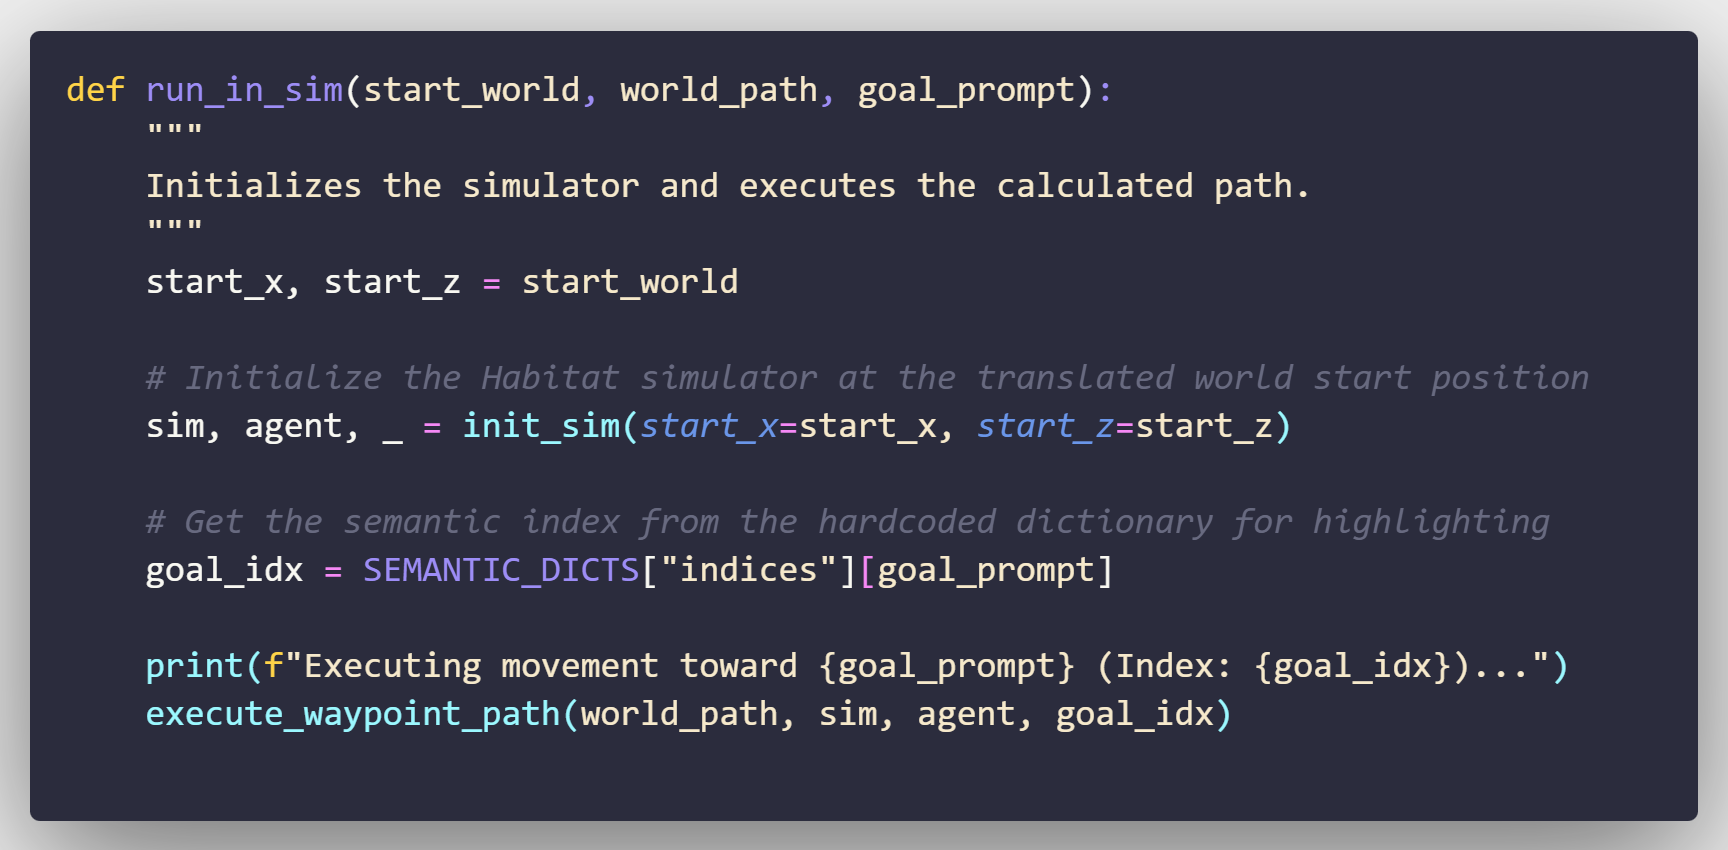
\includegraphics[width=0.9\textwidth]{polacode/run_in_sim.png}
    \caption{Simulation execution logic and navigation control parameters.}
    \label{fig:run_sim}
\end{figure}

The \texttt{run\_in\_sim()} function transforms the abstract list of waypoints into a 
sequence of discrete physical actions within the Habitat environment and displays the navigation result.

\begin{itemize}
    \item \textbf{Simulator Initialization and Configuration:} The \texttt{init\_sim()} 
    function configures the Habitat simulator with three primary sensors: Color (RGB), 
    Depth, and Semantic. The action space is defined with discrete commands: 
    \texttt{MOVE\_FORWARD}, \texttt{TURN\_LEFT}, and \texttt{TURN\_RIGHT}. The agent's 
    starting state is set with the starting point that the user has specified.
    \item \textbf{Two-Phase Navigation Logic:} The \texttt{execute\_waypoint\_path()} 
    function implements a ``turn-then-move'' strategy for each waypoint pair:
    \begin{enumerate}
        \item \textbf{Rotation:} The algorithm calculates the \texttt{target\_angle} to 
        the next waypoint using \texttt{math.atan2(dx, dz)}. The agent then executes a series 
        of 1-degree turns to align its heading with the target vector.
        \item \textbf{Translation:} Once aligned, the agent calculates the number of forward 
        steps required to bridge the distance. 
    \end{enumerate}
    \item \textbf{Precision Tuning with \texttt{MOVE\_AMOUNT}:} A critical improvement I made 
    in this implementation was reducing the \texttt{MOVE\_AMOUNT} parameter from $0.1$ to $0.02$. 
    In discrete simulators, a large step size can cause the agent to ``overshoot'' a waypoint, 
    leading to cumulative errors in position. By utilizing a smaller step size, the agent achieves 
    much higher granular control, ensuring it stays strictly on the planned RRT path even when navigating 
    tight corners or narrow doorways.
    \item \textbf{Visual Feedback and Semantic Highlighting:} The \texttt{navigate\_and\_see()} 
    function provides real-time visualization of the agent's progress. To verify the navigation 
    goal, the function utilizes the \textbf{Semantic Sensor}. When the target object's \texttt{goal\_index} 
    is visible in the agent's field of view, the matching pixels are highlighted via a mask and overlaid with 
    a red color using \textbf{Alpha Blending} (\texttt{cv2.addWeighted}). This creates a semi-transparent 
    "glow" effect, providing visual confirmation that the robot has correctly reached the intended destination.
\end{itemize}

\subsection{Result and Discussion}

In this section, I present the results of the RRT path planning and the subsequent robot 
navigation for three distinct targets: \textbf{Sofa}, \textbf{Cooktop}, and \textbf{Rack}.

\subsubsection{Case 1: Sofa}

\begin{figure}[H]
    \centering
    \begin{minipage}{0.48\textwidth}
        \centering
        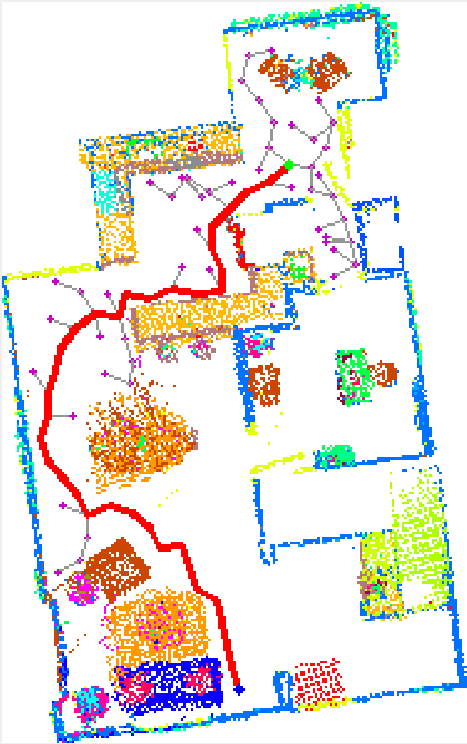
\includegraphics[width=\textwidth]{screenshots/sofa_rrt.png}
        \caption{RRT path for the Sofa.}
    \end{minipage}\hfill
    \begin{minipage}{0.48\textwidth}
        \centering
        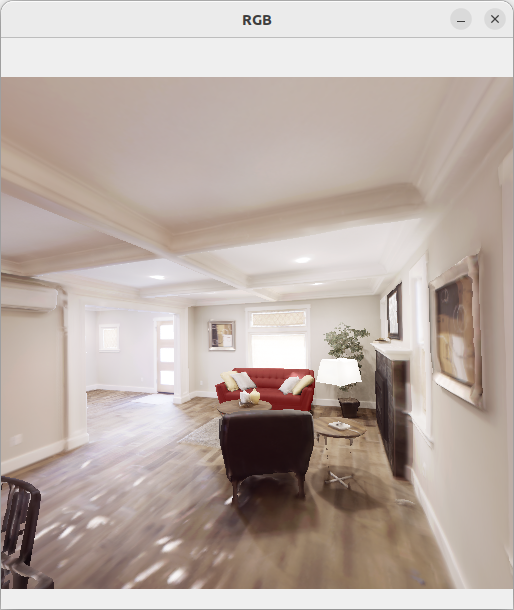
\includegraphics[width=\textwidth]{screenshots/sofa_sim.png}
        \caption{Simulation view with sofa highlighted.}
    \end{minipage}
\end{figure}

\textbf{Discussion:} The RRT map reveals a successful exploration of the living area. 
The 20\% goal bias efficiently directed the tree towards the sofa. Because the path to the 
sofa is relatively wide, the algorithm converged quickly.

\subsubsection{Case 2: Navigation to the Cooktop}

\begin{figure}[H]
    \centering
    \begin{minipage}{0.48\textwidth}
        \centering
        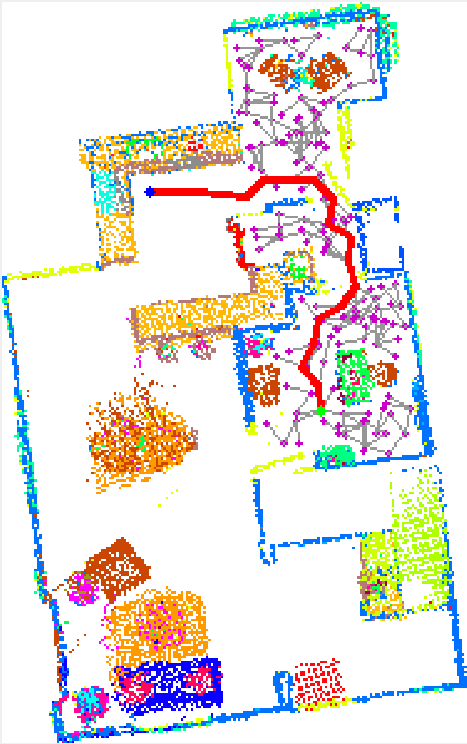
\includegraphics[width=\textwidth]{screenshots/cooktop_rrt.png}
        \caption{RRT path for the Cooktop.}
    \end{minipage}\hfill
    \begin{minipage}{0.48\textwidth}
        \centering
        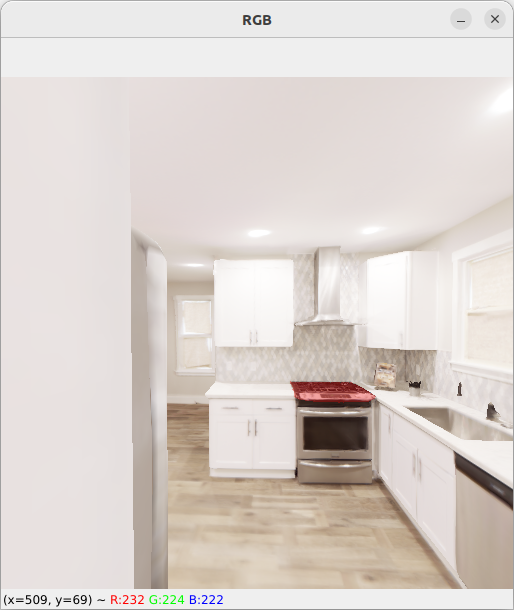
\includegraphics[width=\textwidth]{screenshots/cooktop_sim.png}
        \caption{Simulation reaching the cooktop.}
    \end{minipage}
\end{figure}

\textbf{Discussion:} The RRT tree successfully navigated through the kitchen entrance to 
reach the cooktop. The occupancy grid's dilation was vital here to maintain a safety buffer 
from the kitchen counters. The simulation result shows the agent positioned directly in front 
of the cooktop, with the semantic mask accurately highlighting it.

\subsubsection{Case 3: Navigation to the Rack}

\begin{figure}[H]
    \centering
    \begin{minipage}{0.48\textwidth}
        \centering
        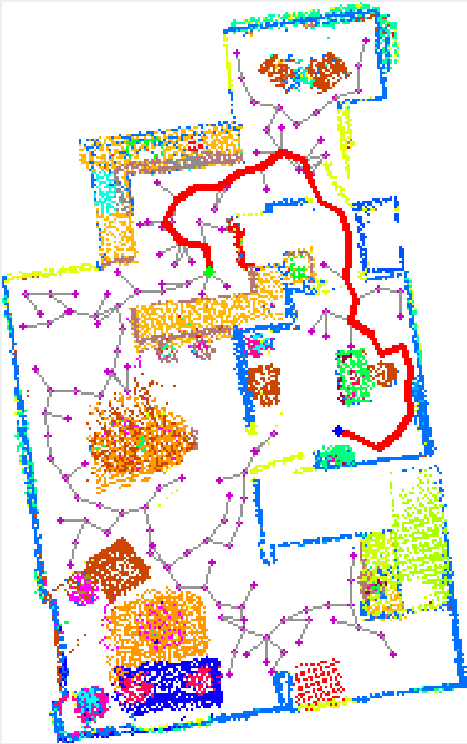
\includegraphics[width=\textwidth]{screenshots/rack_rrt.png}
        \caption{RRT path for the Rack.}
    \end{minipage}\hfill
    \begin{minipage}{0.48\textwidth}
        \centering
        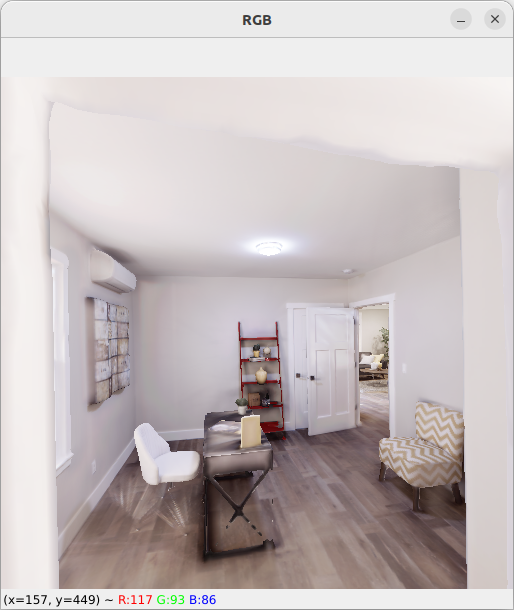
\includegraphics[width=\textwidth]{screenshots/rack_sim.png}
        \caption{Visual confirmation of the rack goal.}
    \end{minipage}
\end{figure}

\textbf{Discussion:} The rack presents a specific challenge as it is located in a rather small 
and narrow room. The \texttt{find\_navigable\_goal} function effectively used the distance transform 
to find a floor point that was close to the rack's centroid and is also reachable (not in a obstacle 
nor on the other side of the room).

\subsubsection{Overall Performance Discussion}

\begin{itemize}
    \item \textbf{Efficiency of RRT with Goal Biasing:} The 20\% goal bias have saved up the number of 
    iterations needed to find a path compared to a purely random sampling approach. It allowed the tree 
    to grow towards the destination while still providing enough exploration to bypass obstacles.
    \item \textbf{Importance of Control Granularity:} Reducing the \texttt{MOVE\_AMOUNT} to $0.02m$ was 
    essential for smooth navigation. This smaller step size allowed the agent to follow the RRT waypoints 
    precisely, preventing the overshooting that might occur with the default $0.1m$ step size.
\end{itemize}

\section{Questions}

\subsection{(a) RRT Parameters: Step Size and Goal Bias}

In the RRT algorithm, the sampling behavior and search efficiency are mainly affected 
by two hyperparameters: \textbf{Step Size} and \textbf{Goal Bias}.

\begin{enumerate}
    \item \textbf{Step Size:} This defines the maximum distance between a new node and 
    its nearest neighbor in the tree.
    \begin{itemize}
        \item \textbf{Exploration Speed:} A large step size allows the tree to ``jump'' across 
        open spaces quickly, reaching the goal in fewer iterations. However, if the step size 
        is too large, the algorithm may fail to navigate through narrow corridors or small 
        doorways because the new node might land inside an obstacle or jump over a valid opening.
        \item \textbf{Precision:} A small step size (like the 10 pixels used in this implementation) 
        provides high precision, allowing the tree to pierce through tight gaps. The trade-off 
        is a significantly higher computational cost, as many more nodes are usually required to 
        cover the same real-world distance.
    \end{itemize}

    \item \textbf{Goal Bias:} This is the probability of selecting the target goal as the random 
    sample instead of a uniform random point in the environment.
    \begin{itemize}
        \item \textbf{Exploitation (High Bias):} A high bias (e.g., $>50\%$) makes the algorithm greedy. 
        The tree grows aggressively toward the goal, which is extremely efficient in obstacle-free 
        environments. However, in complex layouts, high bias often leads to the tree getting stuck 
        in local minima, such as U-shaped furniture or dead-end rooms, because it lacks the curiosity 
        to explore the paths that seems to lead away from the goal to find an opening.
        \item \textbf{Exploration (Low Bias):} A low bias ensures the tree expands uniformly, filling 
        the entire searchable space. While this is slower to converge on a specific target, it is far 
        more robust at finding paths around complex obstacles. My implementation utilized a 
        \textbf{20\% bias}, which provided a healthy balance: the tree prioritized the target while 
        retaining enough randomness to navigate around the apartment's furniture.
    \end{itemize}
\end{enumerate}

\subsection{(b) Real-World Implementation Challenges}

Transitioning an indoor navigation pipeline from a well developed simulator like Habitat-Sim 
to a physical robot involves several critical challenges:

\begin{enumerate}
    \item \textbf{Sensor Noise and Data Sparsity:} Unlike the clean point cloud files used here, 
    real-world depth sensors usually suffer from noises. Transparent surfaces (glass doors), 
    reflective materials (mirrors), and dark objects can create hole-like regions in the point cloud, 
    leading to false obstacles or invisible walls.
    \item \textbf{Localization Drift:} In simulation, we have access to the Ground Truth position. 
    In reality, robots rely on wheel odometry and IMUs, which accumulate error over time. This drift 
    means the robot's estimated position on the 2D map will eventually diverge from its actual physical 
    location as time goes by, requiring the integration of \textbf{SLAM (Simultaneous 
    Localization and Mapping)} to correct its pose.
    \item \textbf{Dynamic Environments:} The current framework assumes a static world. In a 
    real home, the environment is dynamic: people walk, pets move, and chairs are shifted. A 
    real-world pipeline requires a Local Planner to supplement the RRT, allowing the robot to 
    reactively dodge moving obstacles that were not present in the initial 3D scan.
    \item \textbf{Computational Constraints:} Real-time processing of high-density 3D point clouds and 
    RRT iterations requires significant CPU/GPU computational power. On a mobile robot with limited 
    battery and edge-computing hardware, the perception pipeline must be highly optimized to maintain a 
    responsive control loop.
\end{enumerate}

\end{document}